\documentclass[a4paper,11pt]{report}
\usepackage[french]{babel}
\usepackage[T1]{fontenc}
\usepackage[utf8]{inputenc}
\usepackage{lmodern}
\usepackage{microtype}
\usepackage{hyperref}
\usepackage{tabulary}
\usepackage{framed}
\usepackage{fancyhdr}
\usepackage{amsmath}
\usepackage{bbm}
\usepackage{graphicx}

\newcommand{\latin}[1]{\textit{#1}}

\pagestyle{empty}

\pagestyle{fancy}
\fancyhead{}
\renewcommand{\headrulewidth}{0.5pt}
\fancyhead[L]{\textit{\nouppercase{\leftmark}}}
\fancyfoot{}
\renewcommand{\footrulewidth}{0.5pt}
\fancyfoot[R]{\thepage}

\begin{document}
	\begin{titlepage}
		\vspace*{\stretch{2}}
		\begin{center}
			\large\bfseries\itshape Projet SPECIF\\
		\end{center}
		\noindent\rule{\linewidth}{3pt}

		\begin{center}
			\Huge\bfseries\itshape RAPPORT\\
		\end{center}
		
		\noindent\rule{\linewidth}{3pt}
		\begin{center}
			\bfseries
			\large Modèlisation le protocole avec la perte de message
			
		\end{center}
		\vspace*{\stretch{2}}
		\begin{center}
			Réalisé par \bfseries \itshape DOAN Cao Sang
		\end{center}
		\begin{center}
			17 Avril 2015
		\end{center}
	\end{titlepage}

\chapter{Propriété}
	{\huge \itshape L}e programme doit satisfaire les propriétés suivantes:
		\begin{enumerate}
			\item Il n'y a jamais qu'un seul signal électrique sur ce cable principal.
			\item Deux interlocuteurs ne peuvent obtenir le cable en même temps.
			\item En l'absence de pertes, le système ne se bloque pas.
			\item Un message émis arrive toujours à destination.
		\end{enumerate}
	
\chapter{Explication}

	\begin{figure}[!htbp]
		\centering
		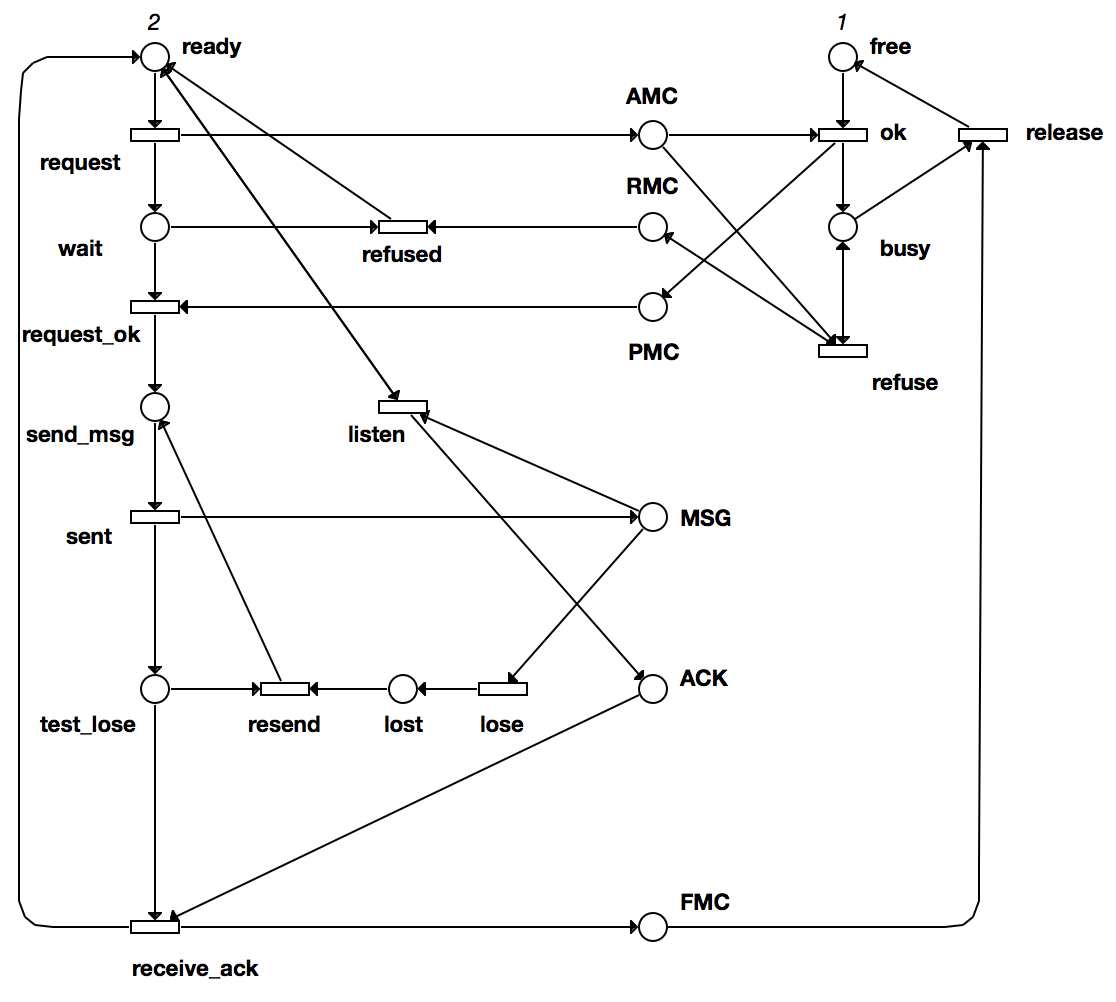
\includegraphics[width = 15cm]{protocole1.png}
		\caption{Le schéma de protocole}
	\end{figure}
	
	{\huge \itshape L}ors que un interlocuteur a acquérit le bus principal, il envoie un message au l'autre, soit le message arrive au destinataire, soit le message se tombe dans un puits. Dans le $1^{er}$ cas, l'émetteur reçoit un ACK au bout un certain temps arbitraire dès que le récepteur reçoit le message mais fini. Dans le $2^{ème}$ cas, si l'émetteur détecte la perte, il renvoie le message jusqu'à quand il est sûr qu'il n'y a pas de perte de message.
	
	\begin{figure}[!htbp]
		\centering
		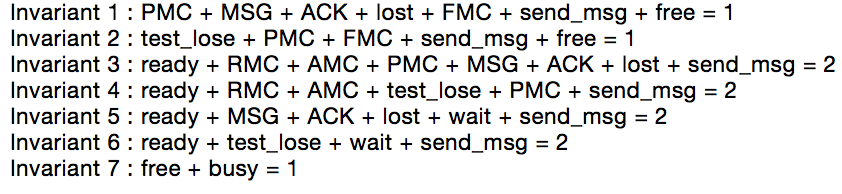
\includegraphics[width = 15cm]{place_invariant.png}
		\caption{Les invariants de places}
	\end{figure}
	
	Selon les invariant ci-dessous, on peut trouver les invariants qui assurent les propriétés demandées sont:
	
		\begin{itemize}
		\item \textit{Invariant 7}: Le cable principal soit occupé, soit libre, donc qu'il ne peut jmais à la fois libre et occupé.
		\item \textit{Invariant 1}: A un instant quelconque, il n'y a qu'un seul message( MSG ou ACK) en transit.
		\item \textit{Invariant 3}: Deux interlocuteurs sont soit dans l'état d'écoute le MSG et envoie ACK quand il reçoit le MSG, soit dans l'état d'émission du MSG, si le MSG est perdu, il doit renvoyer au récepteur.
		\item \textit{Invariant 5}: Cet invariant assure que la $1^{ère}$ propriété a été validé, il y a toujours un ACK suivi du MSG.
	\end{itemize}
	
	\begin{figure}[!htbp]
		\centering
		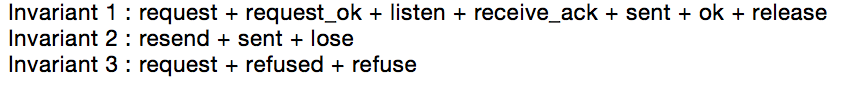
\includegraphics[width = 15cm]{transition_invariant.png}
		\caption{Les invariants de transitions}
	\end{figure}
	
\end{document}





















